\documentclass{beamer}
\usepackage{tikz}
\usepackage{graphicx}
\usepackage{tabu}
\usepackage{fontawesome}
\usetikzlibrary{positioning}
\usetikzlibrary{calc}
%\usetikzlibrary{arrows}

\usefonttheme{professionalfonts}
\usetheme{Boadilla}
\setbeamertemplate{navigation symbols}{}%remove navigation symbols
\hypersetup{pdfstartview={Fit}} % fits the presentation to the window when first displayed
\graphicspath{{./figures/}{./figures/generated/}{./figures/static/}}

%Edwards PB, Wanjura WJ, Brown WV: Selective herbivory by Christmas beetles in response to intraspecific variation in Eucalyptus terpenoids. Oecologia 1993, 95:551–557

%Info
\title[Eucalyptus Somatic Mutation]{Calculating a non-model \textit{Eucalyptus} Individual's Somatic Mutation Rate}
\titlegraphic{
	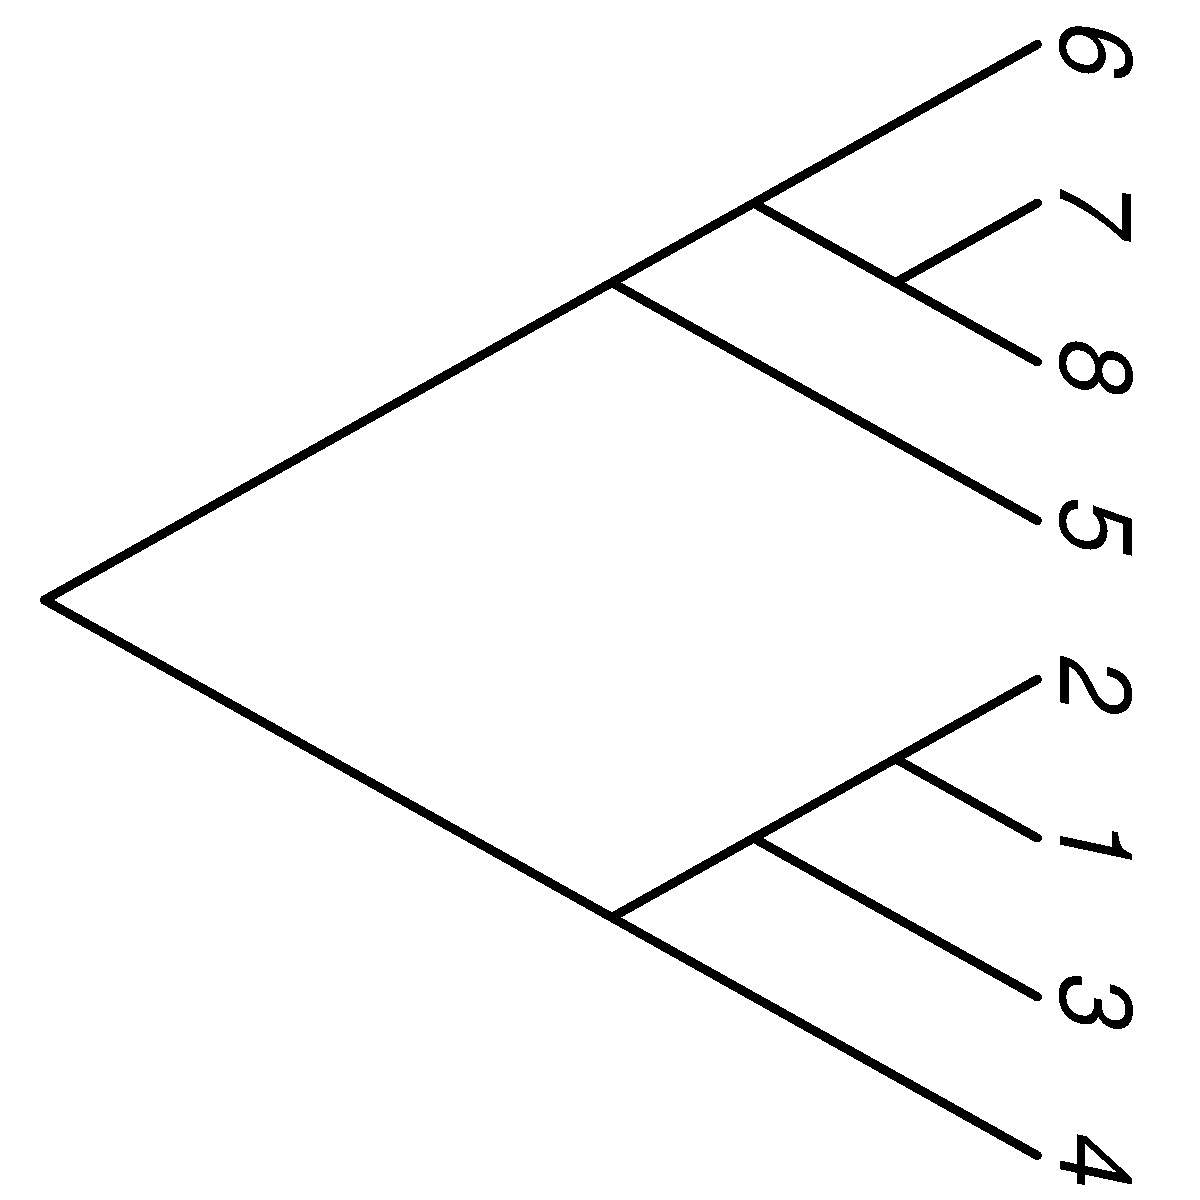
\includegraphics[width=.3\linewidth]{gatk_tree_rightwards.pdf}
	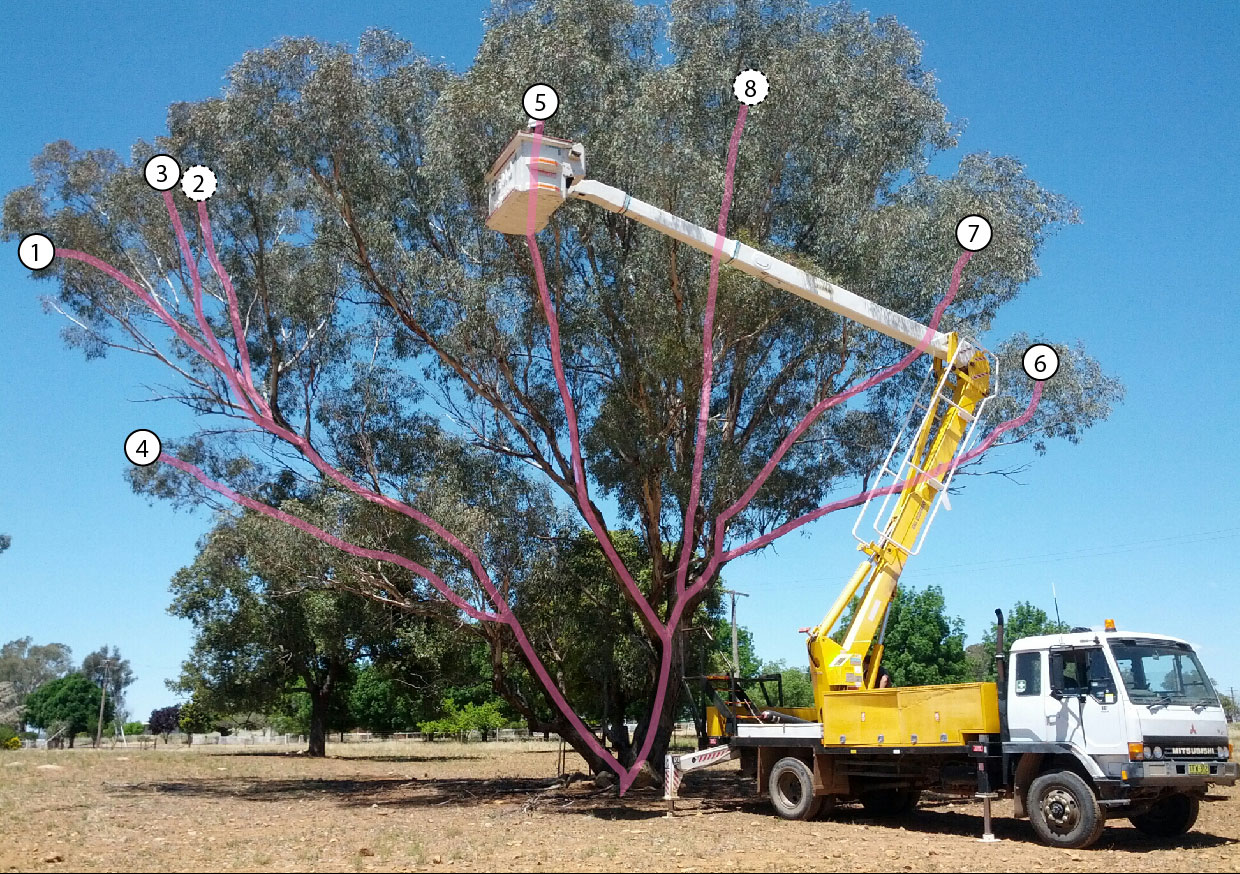
\includegraphics[width=.3\textwidth, angle=90]{labeled_tree.jpg}
	}
\date{9/25/18}
\author{Adam Orr\hskip 1em \faicon{twitter}@AdamJOrr}

\begin{document}
\frame{\titlepage}

% \begin{frame}{Why look for somatic mutations?}
% 	\begin{tabu} to .95\textwidth { X[c] | X[c] }
% 	% row 1 col 1
% 	\textbf{Disease} & \textbf{Development}
% 	\\
% 	Cancer \& Somatic mutation rate & Understanding relationship between tissues
% 	\\
% 	\\
% 	\hline
% 	\\
% 	\textbf{Agriculture} & \textbf{Evolution}
% 	% row 2 col 1
% 	\\
% 	Looking for interesting phenotypes in clonally reproducing species & Relationship between somatic and germline mutation rate. Evolution of mutator phenotypes. Mutational stress response.
% 	\end{tabu}
% \end{frame}

\begin{frame}{Somatic Mutations Occur During Replication Even Without Exposure to Mutagens}
\begin{columns}
	\column{.65\linewidth}
		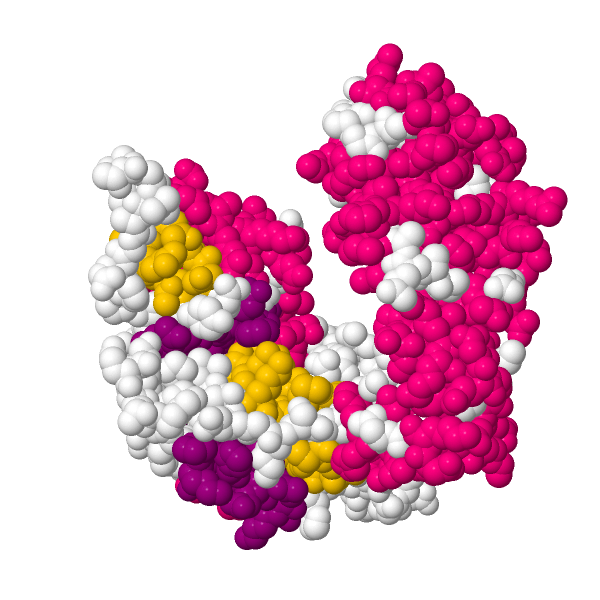
\includegraphics[width=\linewidth]{dnapol_beta.png}
	\column{.35\linewidth}
		\begin{itemize}
			\item DNA Polymerase $\beta$
			\item Mutation rate $\sim10^{-9}$
		\end{itemize}
		\vskip 3in
		\footnotetext{PDB: 7ICG}
\end{columns}
\end{frame}

\begin{frame}{Plants Grow Directionally}
\begin{columns}
	\column{.6\linewidth}
		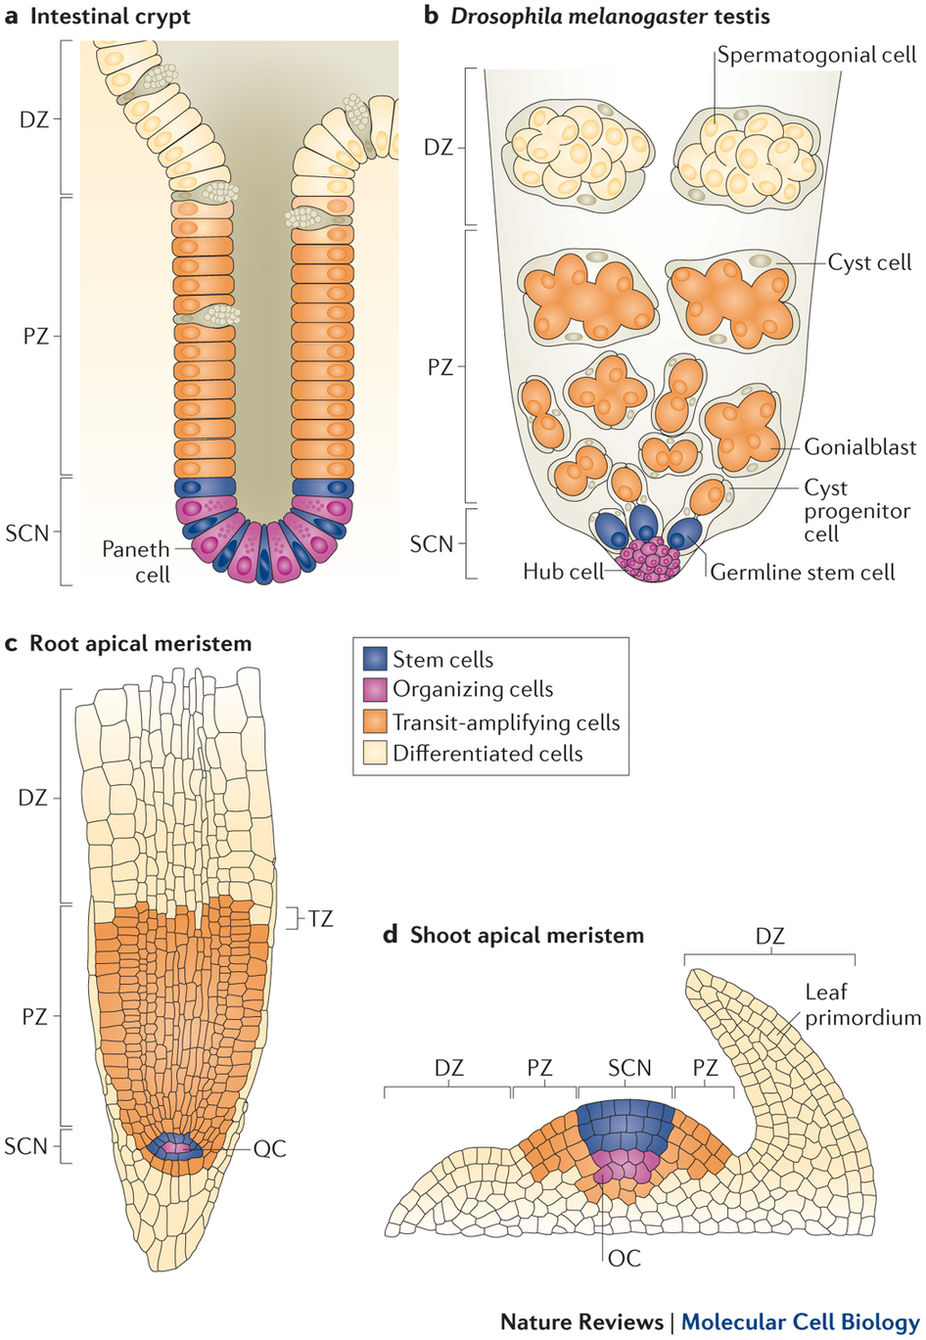
\includegraphics[trim={12cm 2cm 0 22cm},clip,width=\linewidth]{stemcells.jpg}
	\column{.4\linewidth}
		\begin{itemize}
			\item The genetic structure of the plant \textit{should} mirror its physical structure.
		\end{itemize}
\end{columns}
\footnotetext{Heidstra \& Sabatini (2014) Plant and animal stem cells: similar yet different. doi:10.1038/nrm3790}
\end{frame}

\begin{frame}{Do Plants Evolve Differently?}

	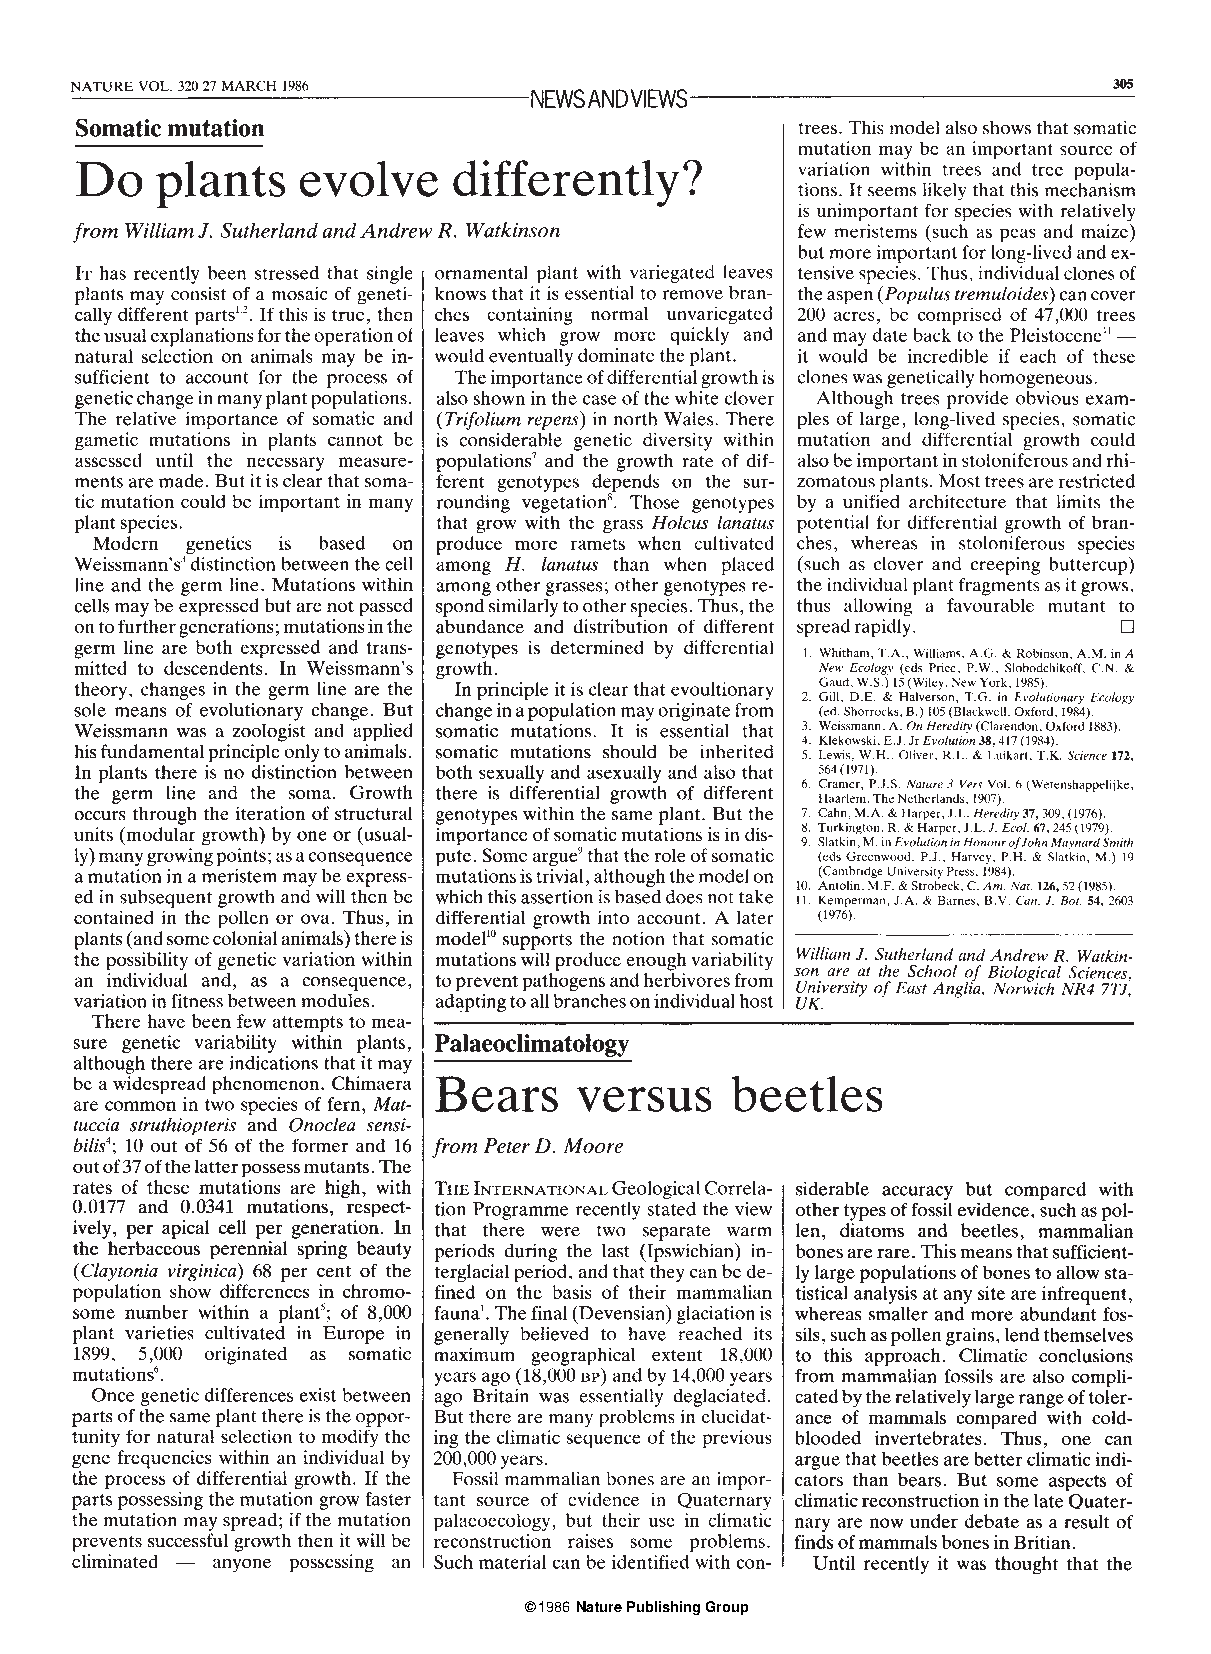
\includegraphics[trim={1.2cm 23cm 1.2cm 0},clip,width=\linewidth]{do_plants_evolve_differently.pdf}

	\vfill

	\begin{columns}
	\column{.5\linewidth}
		\begin{alertblock}{}
			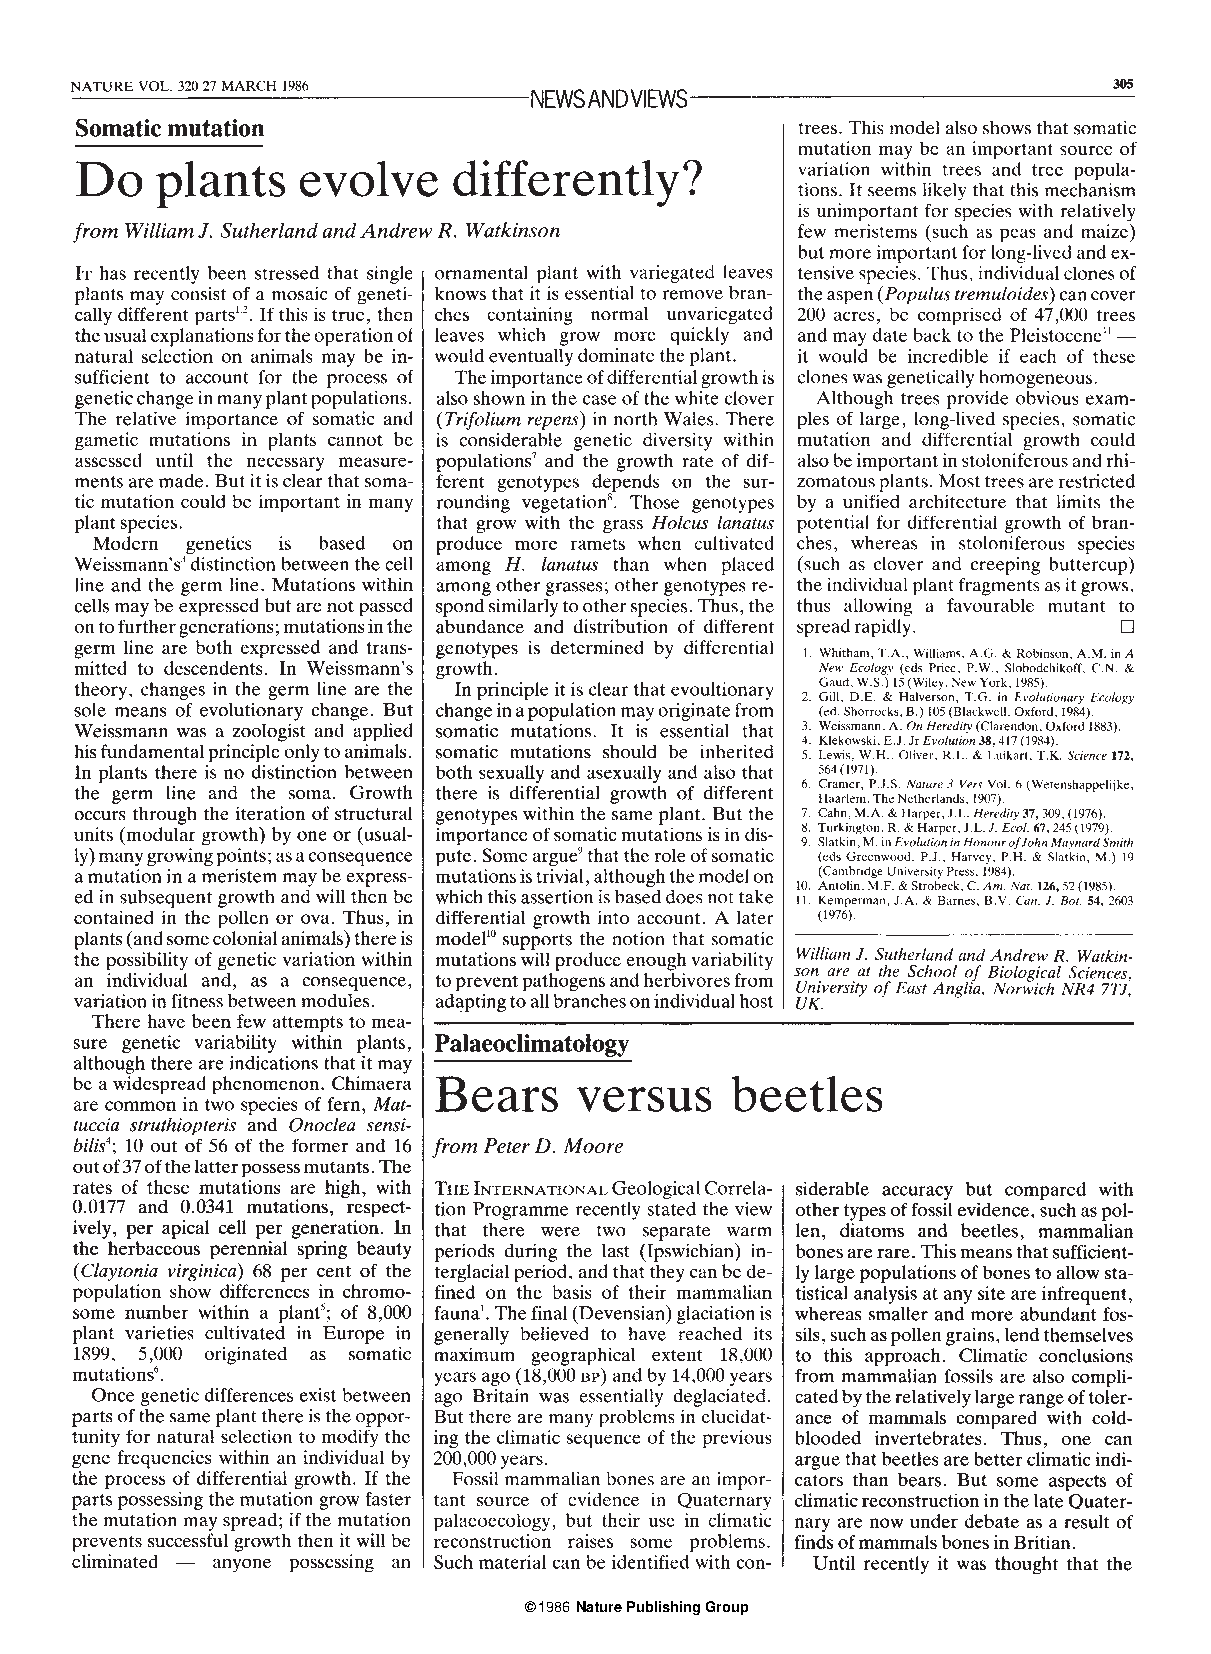
\includegraphics[trim={1.2cm 19cm 13.5cm 6.95cm},clip,width=\linewidth]{do_plants_evolve_differently.pdf}
		\end{alertblock}
	\column{.4\linewidth}
		Plants are weird.
		\begin{itemize}
			\item Segregated germline?
			\item Dedifferentiation
			\item Selfing
			\item Mutational stress response?
		\end{itemize}


	\end{columns}

	% Plant genomes are weird.

	% Genome-level approach required to find enough mutations, but plant genomes are difficult to work with due to highly repetitive genomes.

	% \vfill

	% Relatively few plant genomes.

	% \begin{itemize}
	% 	\item Do plants have a segregated germline?
	% 	\item Do plants induce mutation in response to stress?
	% how significant of a contribution do somatic mutations play in gamete production?
	% \end{itemize}

	% To answer these questions, we must first have methods to sensitively detect mutations.

\end{frame}

\begin{frame}{Why are somatic mutations difficult to detect?}

\begin{block}{Mutations are very rare, but sequencing errors are very common.}
\textbf{Sequencing error} alone is \textbf{$\sim10^{-2}$} while mutation rate after error-checking is \textbf{$\sim10^{-9}$}
\end{block}

\begin{itemize}
\item Errors accumulate during PCR prior to sequencing - then propagate.
\item \textit{Taq} $\sim10^{-4}$
\item Technical error from sequencer
\end{itemize}

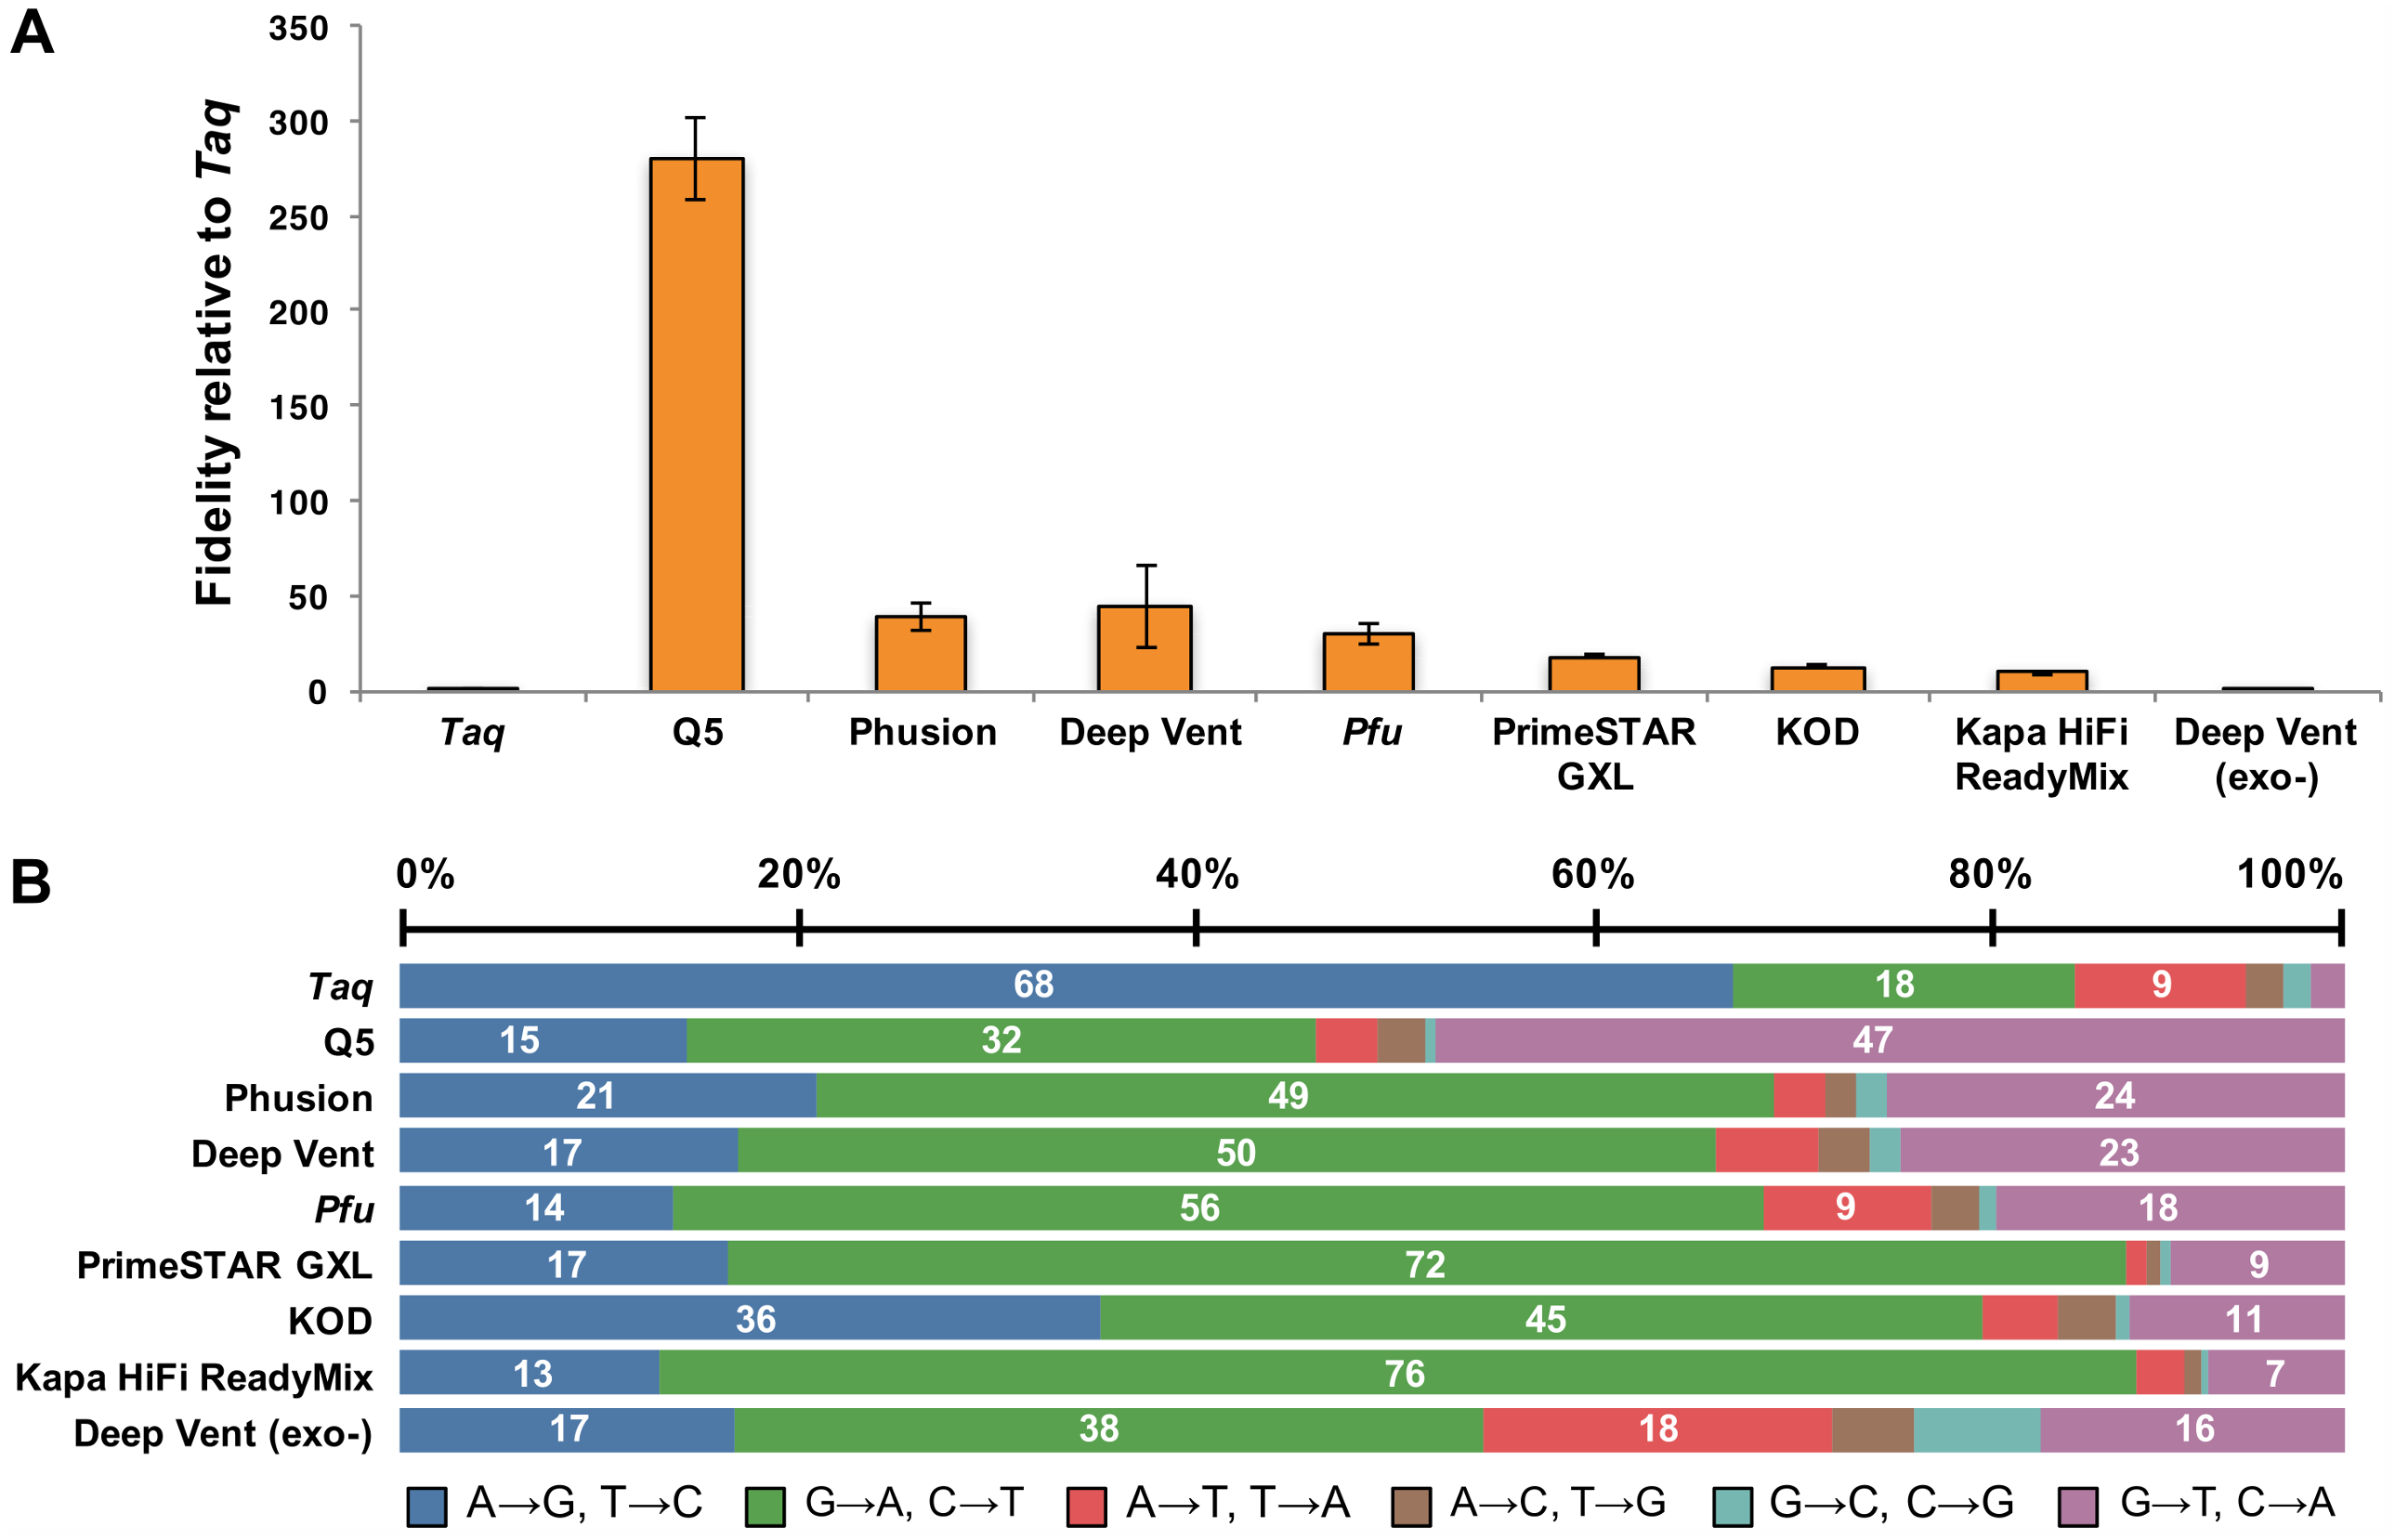
\includegraphics[trim={1cm 4cm 0 0},clip,width=\linewidth]{pcr_errors.png}

\footnotetext{\tiny{Potapov V, Ong JL (2017) Examining Sources of Error in PCR by Single-Molecule Sequencing}}

\end{frame}


\begin{frame}{Why Care About Somatic Mutations?}
\begin{columns}

\column{.5\linewidth}
\textbf{Disease}
\begin{itemize}
\item Cancer
\end{itemize}

\vfill

\textbf{Development}
\begin{itemize}
\item Understanding the relationship between tissues
\end{itemize}

\vfill

\textbf{Agriculture}
\begin{itemize}
\item Looking for interesting phenotypes in clonally reproducing species
\end{itemize}

\textbf{Evolution}
\begin{itemize}
\item Determining the relationship between somatic and germline mutation rate
\end{itemize}

\column{.5\linewidth}
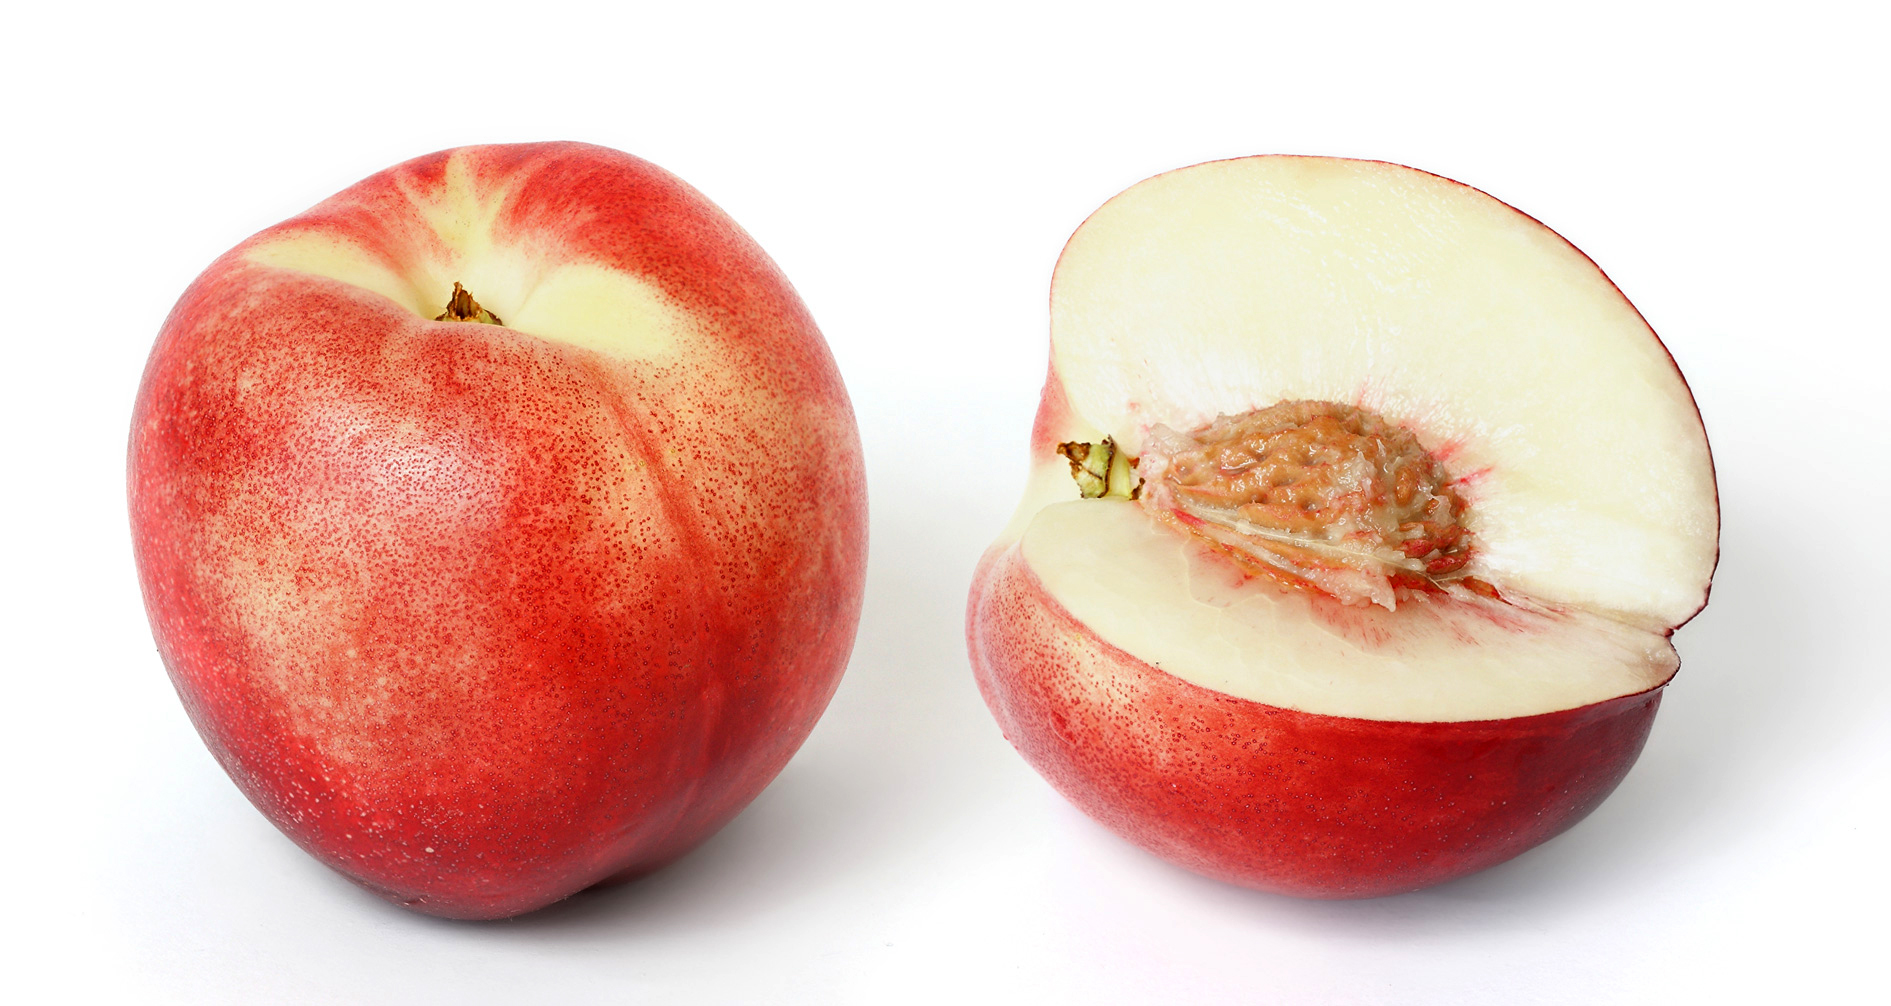
\includegraphics[width=\linewidth]{nectarine.jpg}

\end{columns}
\footnotetext{\tiny{\url{https://commons.wikimedia.org/wiki/File:White_nectarine_and_cross_section02_edit.jpg}}}
\end{frame}

\begin{frame}{Project Goals}

\begin{block}{Is it possible?}
Can we detect mutations with sufficient accuracy to reconstruct the physical structure of a tree?
\end{block}

\begin{exampleblock}{The Relevant Measurements}
What's the mutation rate like? Is there evidence of hypermutation?
\end{exampleblock}

\end{frame}

\begin{frame}{A Genetic Mosaic}
	\begin{center}
	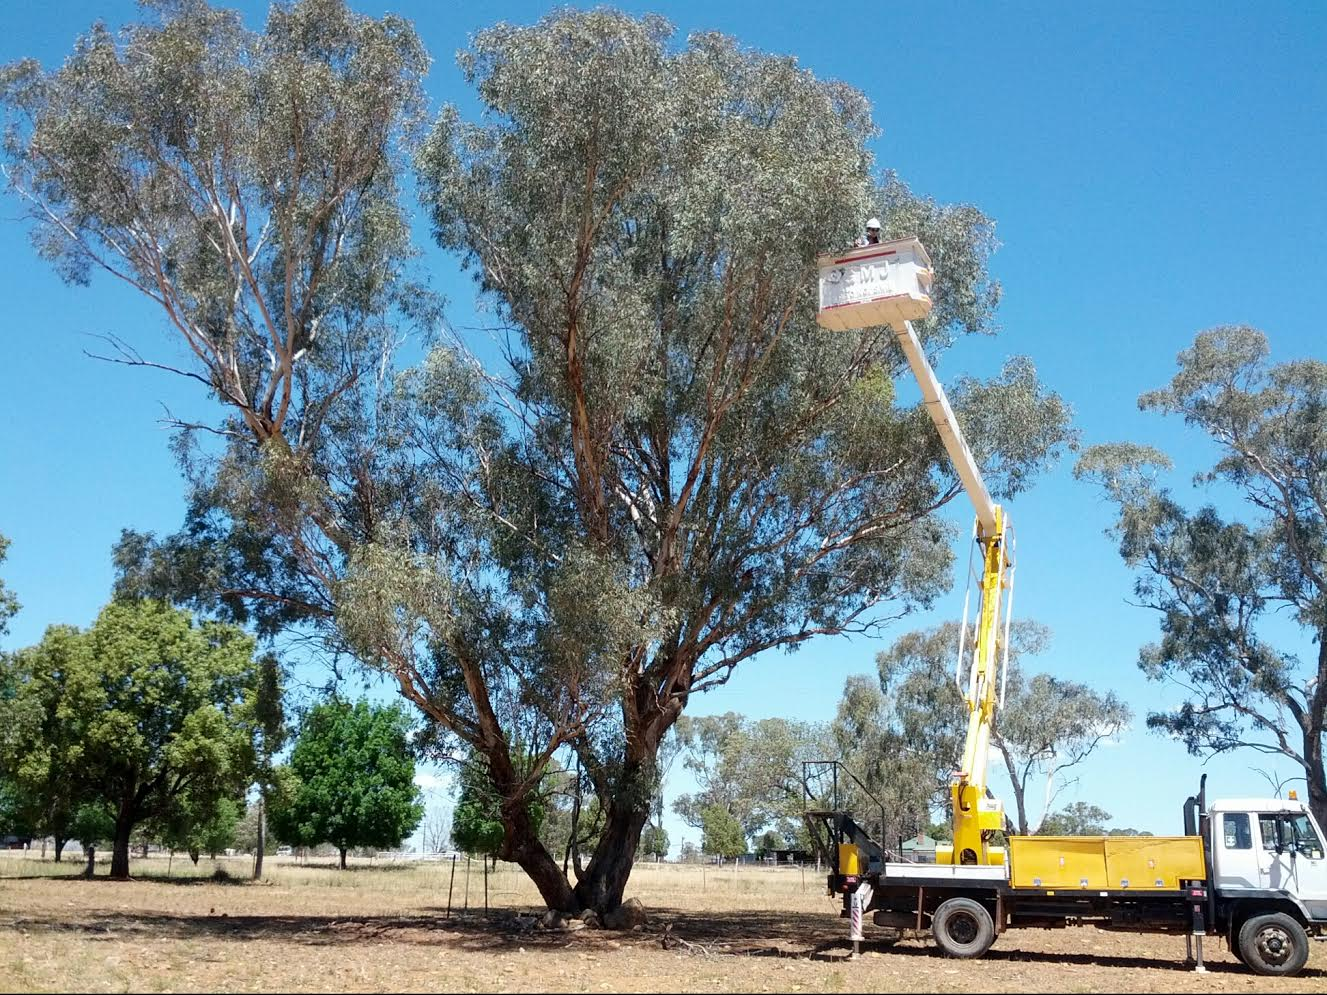
\includegraphics[width=.6\linewidth]{unlabeled_tree.jpg}
	\end{center}
	\begin{itemize}
		\item Edwards identified as mosaic in 1993\footnote{\textit{Edwards PB, Wanjura WJ, Brown WV. Oecologia 1993, 95:551–557.}}
		\item Sheep pen in Yeoval, New South Wales
		\item Differential oil production gives protection from Christmas beetles
		% \item Is this mutation a controlled process?
	\end{itemize}
\end{frame}


\begin{frame}{Study Methodology}
\begin{columns}

\column{.5\linewidth}
\begin{itemize}
\item Sequence 8 samples in triplicate
\item $\sim$10X coverage for each replicate
\item Align sequence to genome of \textit{Eucalyptus grandis}
\item Use replicates to remove false positives
\end{itemize}

\column{.5\linewidth}
\begin{center}
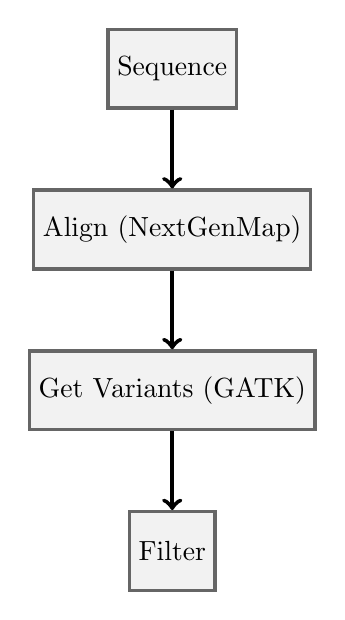
\begin{tikzpicture}[sqnode/.style={rectangle, draw=black!60, fill=black!5,very thick,minimum size=1cm}]
	\node[sqnode] (sequencing) {Sequence};
	\node[sqnode] (alignment) [below = of sequencing] {Align (NextGenMap)};
	\node[sqnode] (varcall) [below = of alignment] {Get Variants (GATK)};
	\node[sqnode] (flt) [below = of varcall] {Filter};
	\draw[ultra thick,->] (sequencing.south) -- (alignment.north);
	\draw[ultra thick,->] (alignment.south) -- (varcall.north);
	\draw[ultra thick,->] (varcall.south) -- (flt.north);
\end{tikzpicture}
\end{center}
\end{columns}
\end{frame}

\begin{frame}{Study Methodology}
\begin{columns}

\column{.5\linewidth}
\begin{itemize}
\item Sequence 8 samples in triplicate
\item $\sim$10X coverage for each replicate
\item Align sequence to genome of \textit{Eucalyptus grandis}
\item Use replicates to remove false positives
\end{itemize}

\column{.5\linewidth}
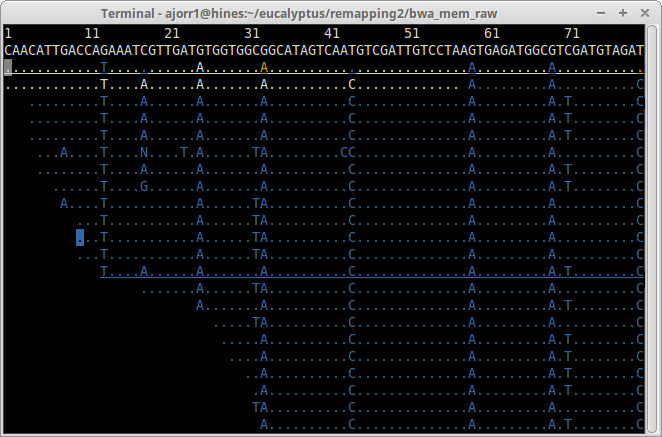
\includegraphics[width=\linewidth]{coverage.png}
\end{columns}
\end{frame}

\begin{frame}{Mutation Pattern Approximately Matches Tree Structure}
\begin{columns}
\column{.5\linewidth}
	\begin{center}
	GATK Best Practices Tree
	\end{center}
	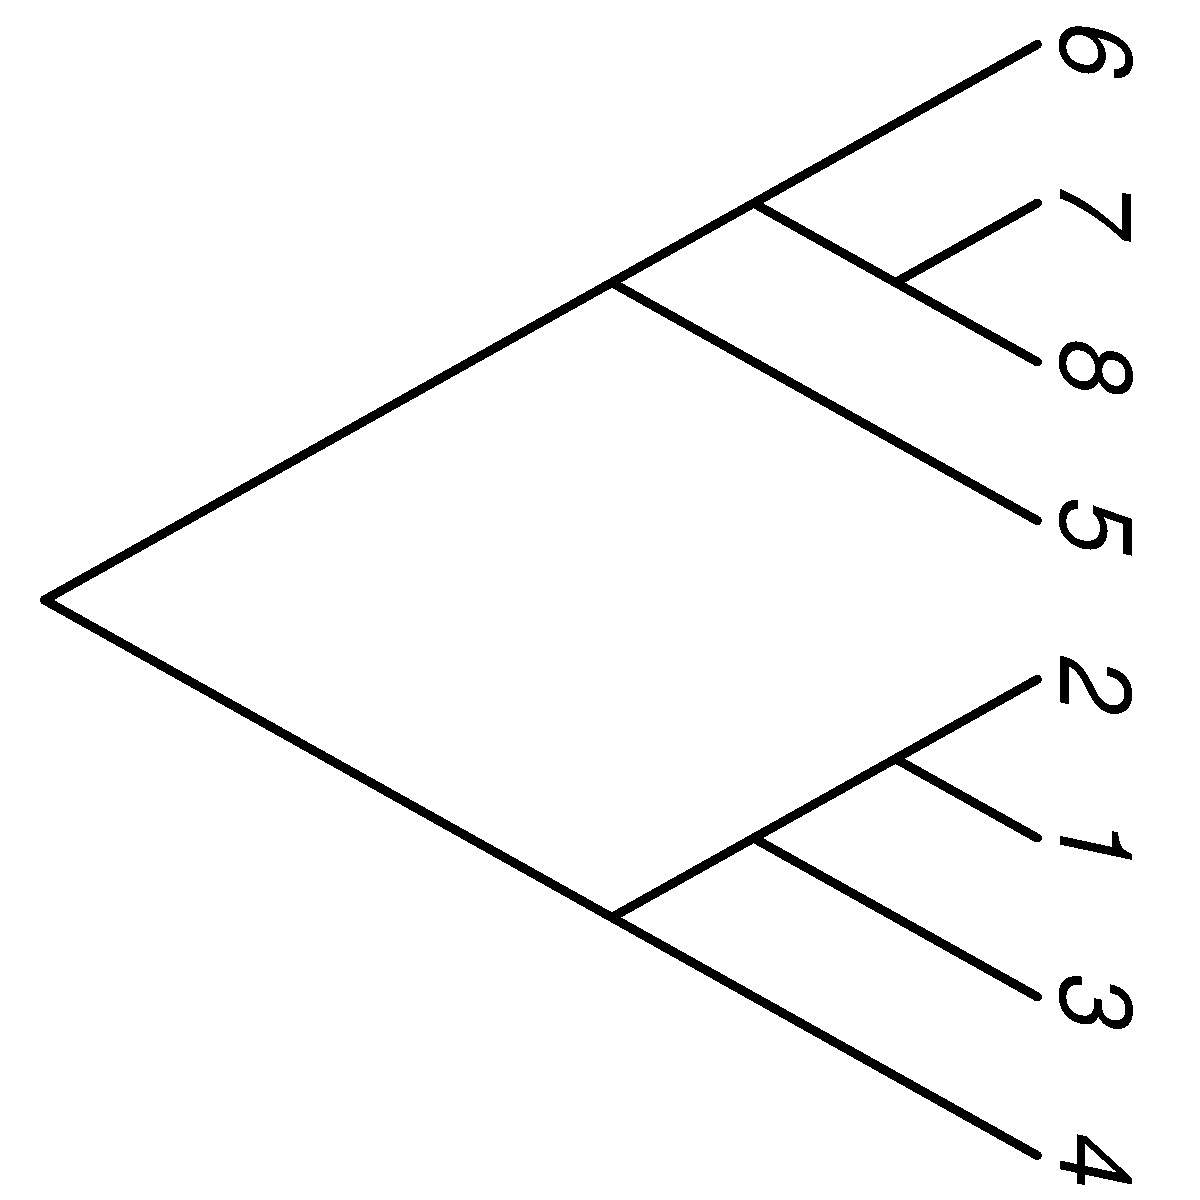
\includegraphics[width=\linewidth]{gatk_tree_rightwards.pdf}
\column{.5\linewidth}
	\begin{center}
	True Tree
	\end{center}
	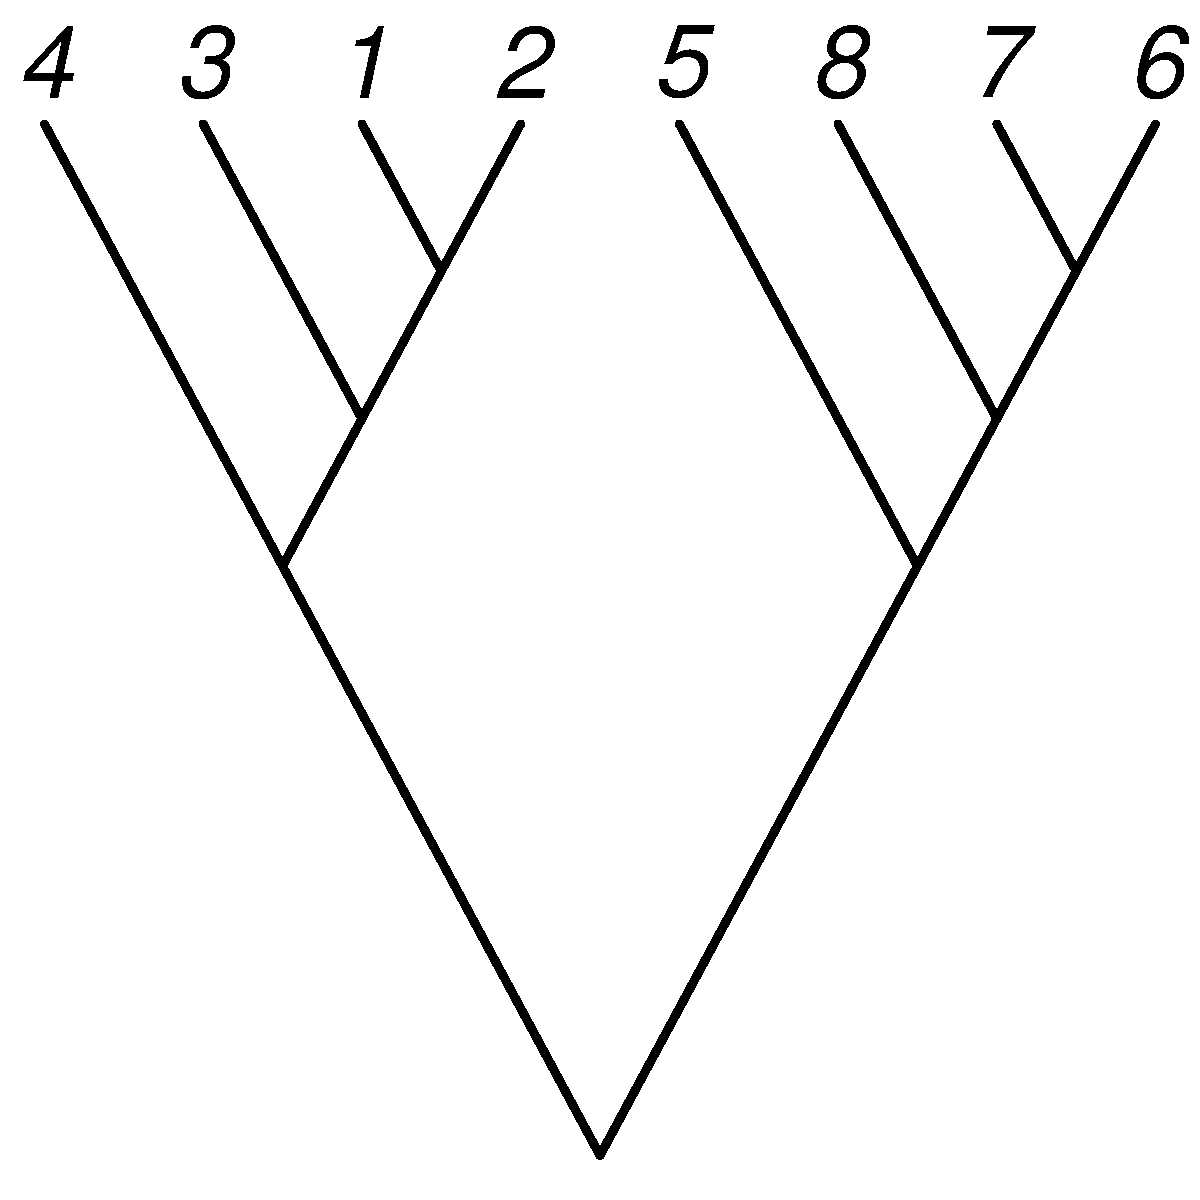
\includegraphics[width=\linewidth,angle=90]{true_tree.pdf}
\end{columns}
\end{frame}

\begin{frame}{Most Reads Are Not Mapped to the \textit{E. grandis} Reference}
\begin{center}
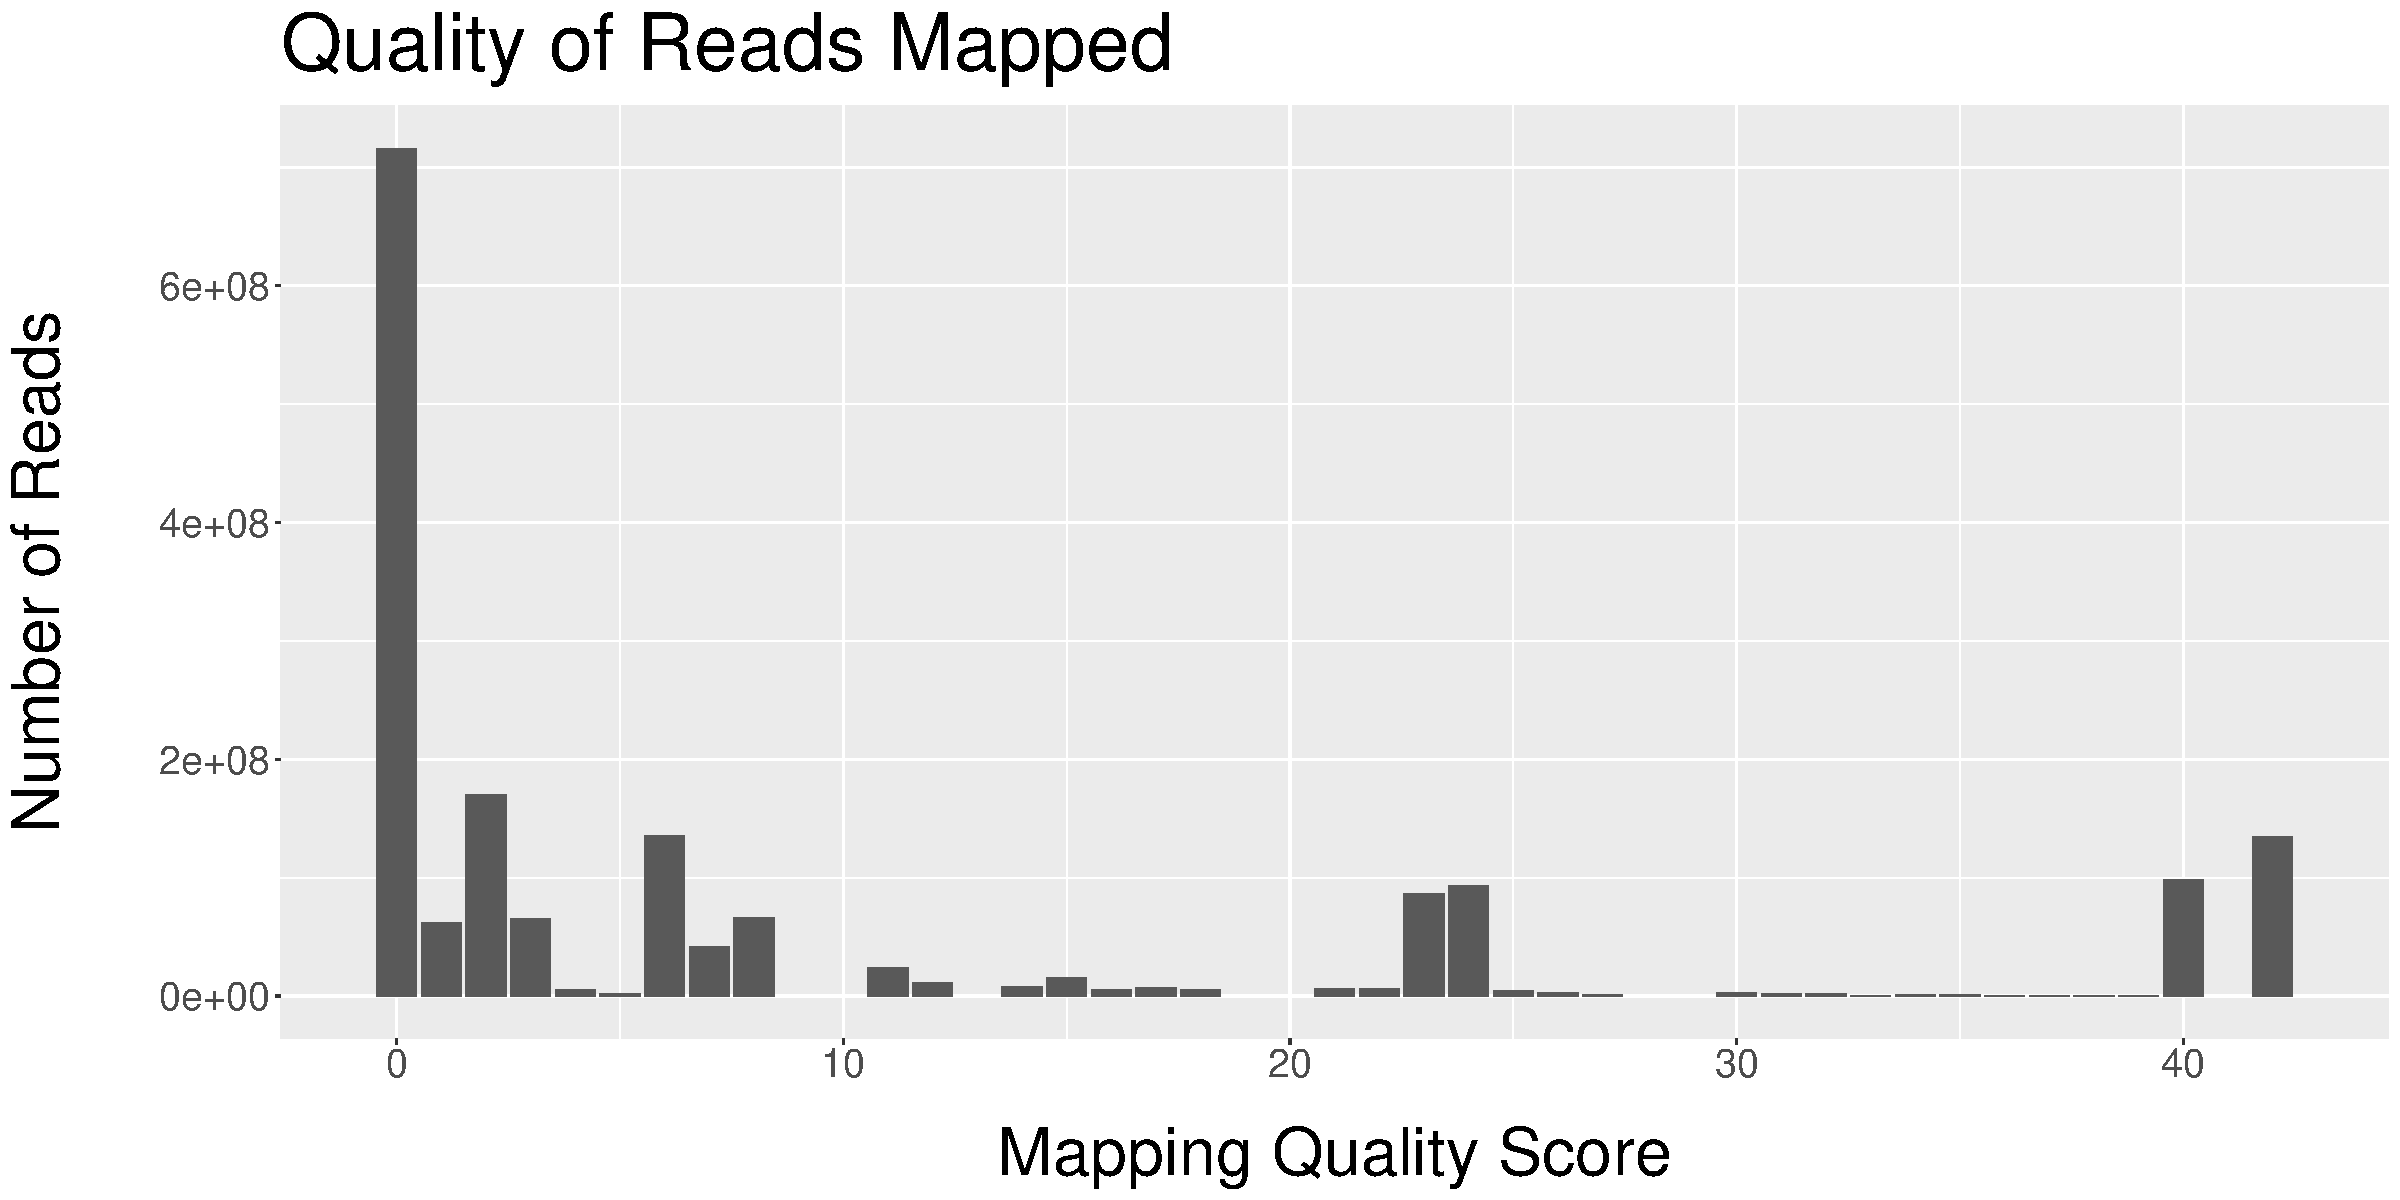
\includegraphics[width=\linewidth]{bowtie1_hist.pdf}
\end{center}
\end{frame}

\begin{frame}{A Reference-Free Method Performs Similarly}
	\begin{columns}
	\column{.5\linewidth}
		\begin{center}
		DiscoSNP++ Tree
		\end{center}
		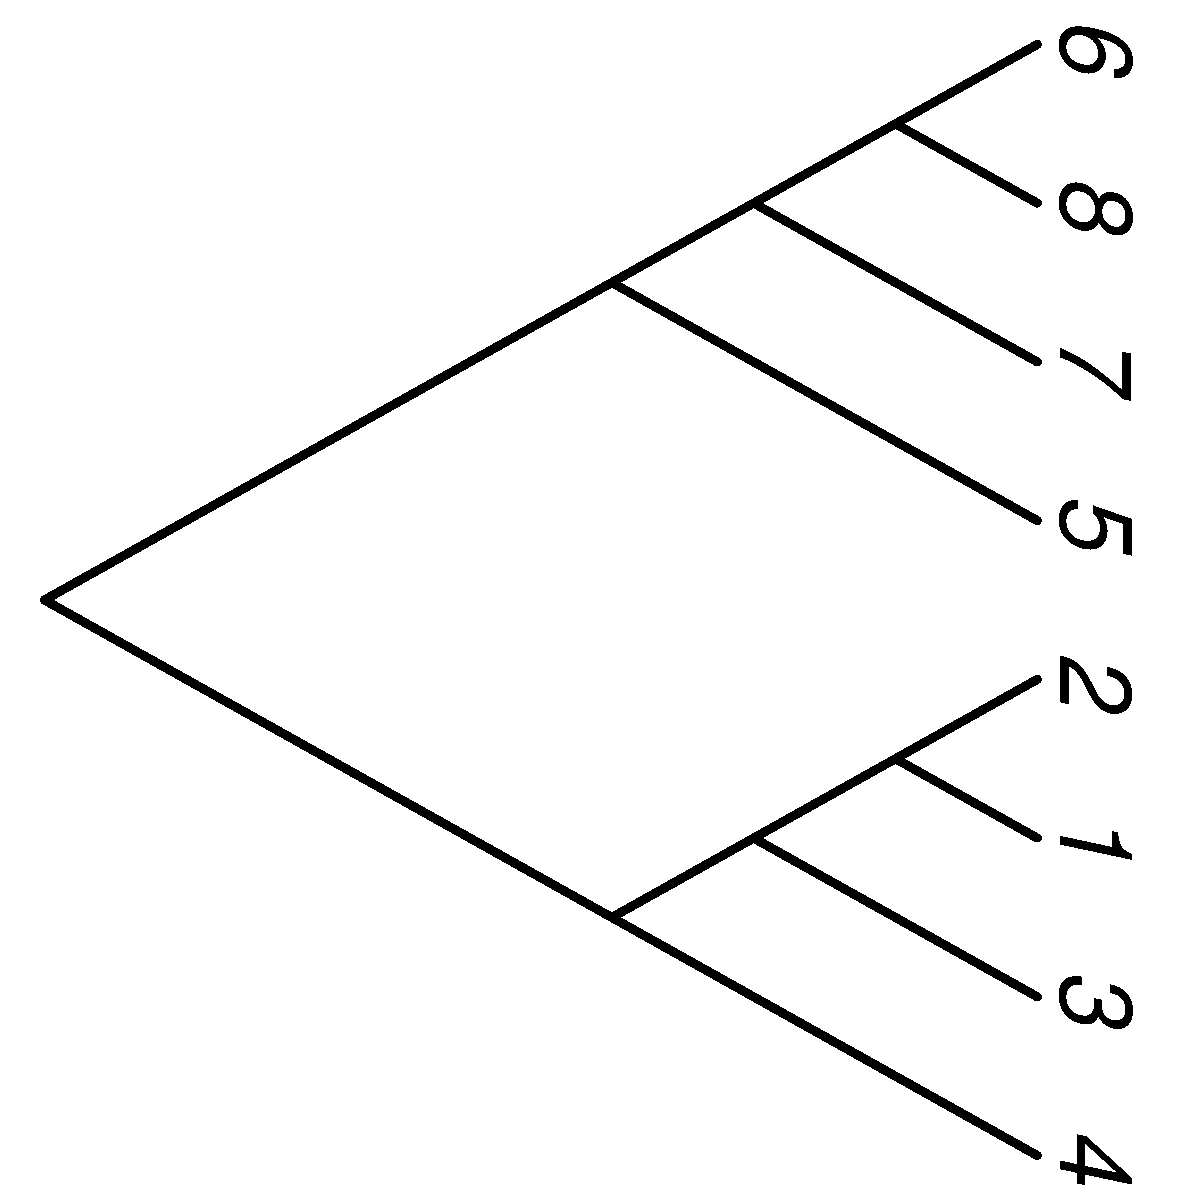
\includegraphics[width=\linewidth]{disco_tree_rightwards.pdf}
	\column{.5\linewidth}
		\begin{center}
		True Tree
		\end{center}
		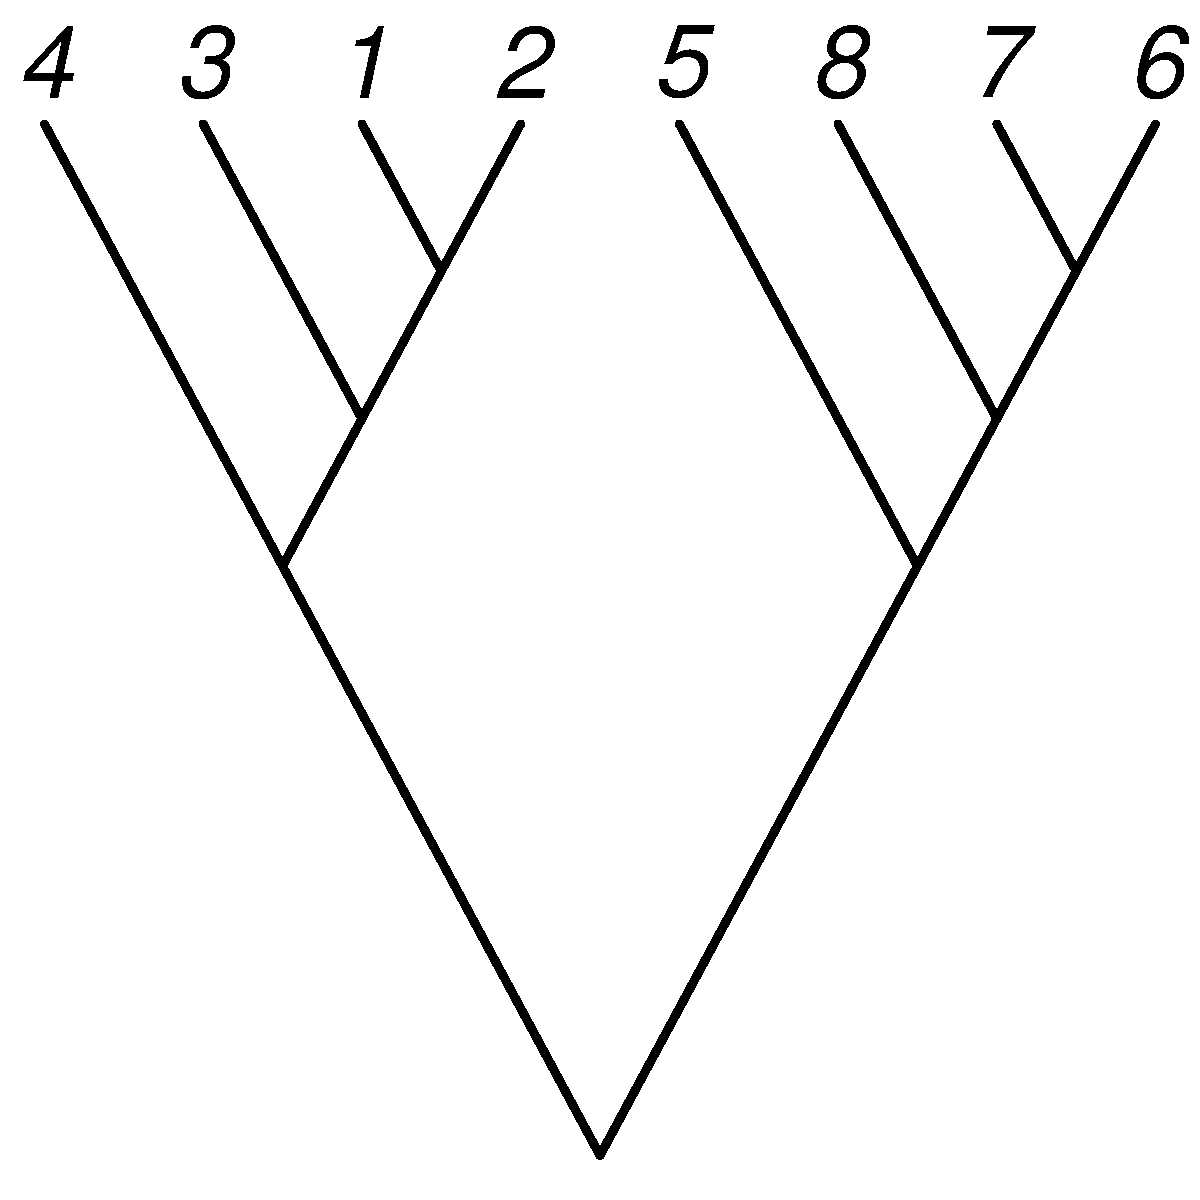
\includegraphics[width=\linewidth,angle=90]{true_tree.pdf}
	\end{columns}
\end{frame}


\begin{frame}{Approximating a Genome}

Use \textit{E. melliodora} genome as a starting place, then generate a new reference and map to that reference.

\begin{center}
	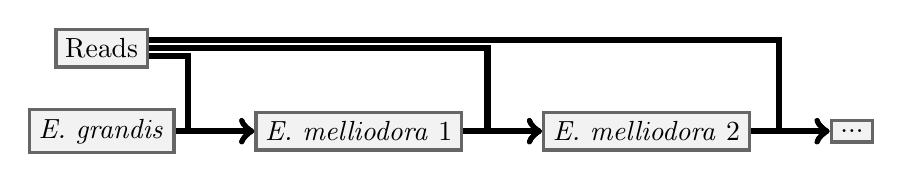
\begin{tikzpicture}[cnode/.style={rectangle,draw=black!60,fill=black!5,very thick}, node distance = 1 cm]
		\node[cnode] (reads){Reads};
		\node[cnode] (eg)[below = .5cm of reads]{\textit{E. grandis}};
		\node[cnode] (em1)[right = of eg]{\textit{E. melliodora} 1};
		\node[cnode] (em2)[right = of em1]{\textit{E. melliodora} 2};
		\node[cnode] (etc)[right = of em2] {...};
		\draw[line width=.8mm,->] ($(reads.east)-(0cm,.1cm)$) -- ($(reads.east)+(.5cm,-.1cm)$) |- (em1.west);
		\draw[line width=.8mm,->] (reads.east) -- ($(reads.east)+(4.3cm,0cm)$) |- (em2.west);
		\draw[line width=.8mm,->] ($(reads.east)+(0cm,.1cm)$) -- ($(reads.east)+(8cm,.1cm)$) |- (etc.west);
		\draw[line width=.8mm,->] (eg) -- (em1);
		\draw[line width=.8mm,->] (em1) -- (em2);
		\draw[line width=.8mm,->] (em2) -- (etc);
	\end{tikzpicture}
\end{center}


\end{frame}

\begin{frame}{Our New Reference Has Fewer Unmapped Reads}
\begin{center}
\includegraphics[width=.95\linewidth]{unmapped_reads.pdf}
\end{center}
\end{frame}

\begin{frame}{Filtering Variants}
\begin{columns}
\column{.5\linewidth}
Remove variants likely from alignment errors:
\begin{itemize}
	\item at sites with excessive depth ($>$500).
	\item with excessive levels of heterozygosity.
	\item within 50 bases of an indel.
	\item in repeat regions 
\end{itemize}
\column{.5\linewidth}
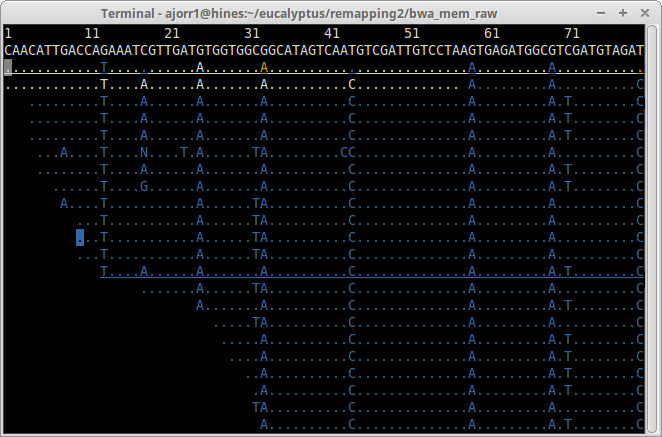
\includegraphics[width=\linewidth]{coverage.png}
\end{columns}
\end{frame}


\begin{frame}{Removing Variants in Repeat Regions Improves Tree Topology}
	\begin{columns}
	\column{.5\linewidth}
		\begin{center}
		Predicted Variants
		\end{center}
		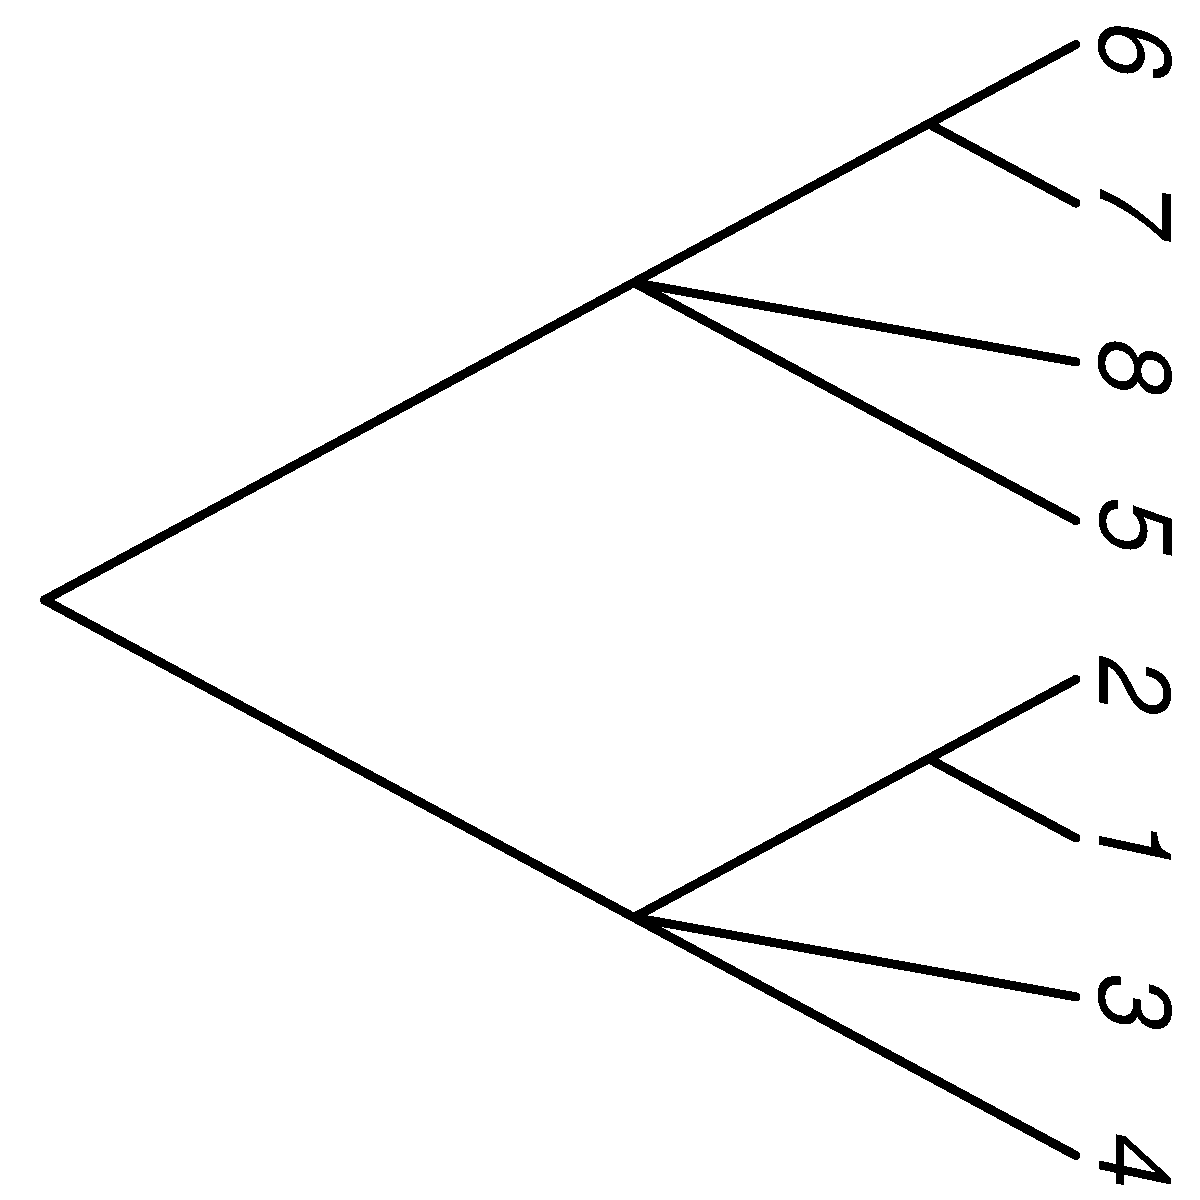
\includegraphics[width=\linewidth]{gatk_repeats_removed.pdf}
	\column{.5\linewidth}
		\begin{center}
		True Tree
		\end{center}
		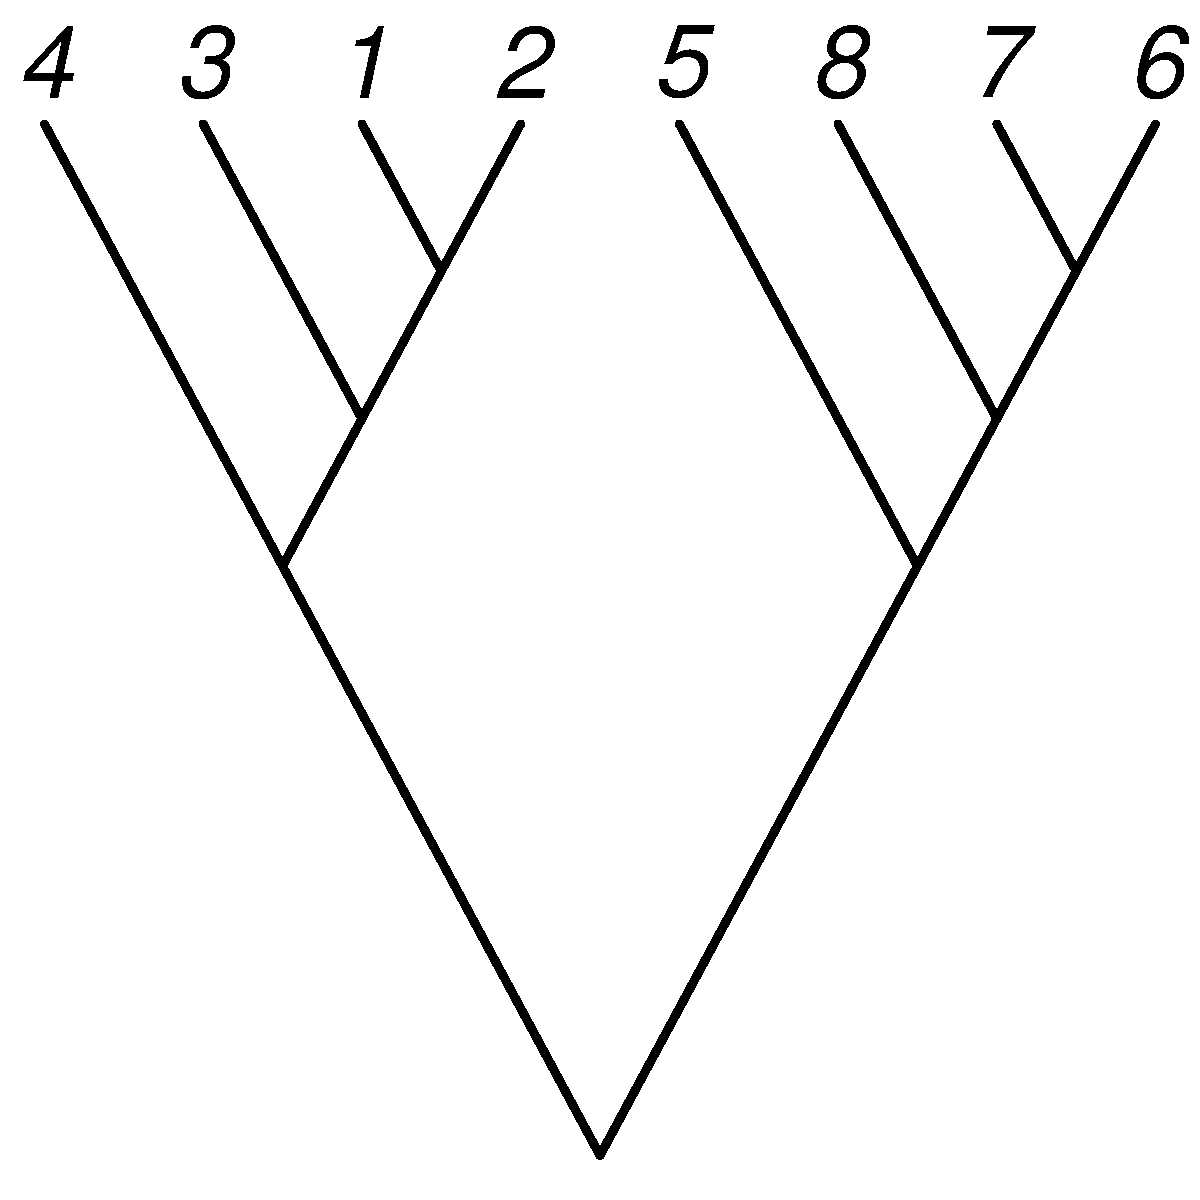
\includegraphics[width=\linewidth,angle=90]{true_tree.pdf}
	\end{columns}
\end{frame}

\begin{frame}{Using Tree Topology Gives Higher Recall Rate}
	\begin{itemize}
	\item \textit{DeNovoGear} is a variant-calling method that uses information in the tree topology to call variants.
	\item By simulation, we introduced 14000 mutations on the tree
	\end{itemize}
	\begin{center}
	\begin{tabular}{ c | c }
	\textit{GATK} & \textit{DeNovoGear} \\
	\hline
	3859 mutations & 4193 mutations \\
	27\% & 30\%
	\end{tabular}
	\end{center}
\end{frame}

% \begin{frame}{Randomizing Trees to Estimate False Positive Rate}
% 	\begin{itemize}
% 		\item Does using a phylogeny increase our false positive rate?
% 		\item Simulate 100 trees maximally distant from the true tree.
% 		\item Does our pipeline detect variation where there shouldn't be any?
% 		\item \textbf{All} sites detected were variable sites.
% 	\end{itemize}
% \end{frame}

\begin{frame}{Mutation Rates}
\begin{columns}
\column{.5\linewidth}
\begin{itemize}
\item Detected $91$ mutations.
\item $20$ mutations in genes.
\item Estimated recall of $\sim30\%$.
\item $91\times\frac{1}{.3}=303$ mutations.
\item $2.5\times10^{-7}$ mutations per site per genome
\item $\sim1.4$ mutations per meter of length
\item Somatic mutations account for $\sim55$ mutations per leaf tip.
\end{itemize}
\column{.5\linewidth}
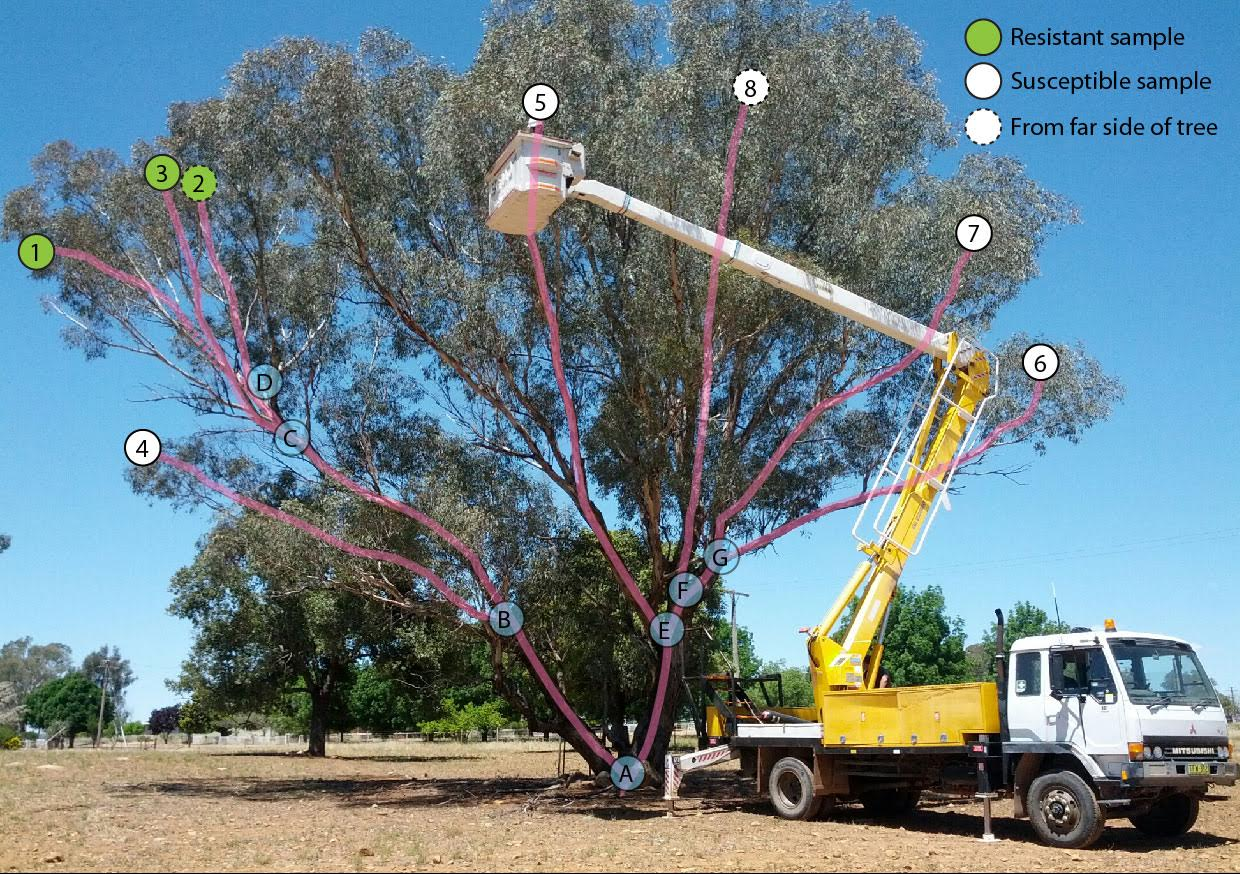
\includegraphics[width=\linewidth]{labeled_nodes_tree.jpg}
\end{columns}
\end{frame}


\begin{frame}{Acknowledgements}
\begin{itemize}
\item Advisor: Reed Cartwright\hskip 1em \faicon{twitter}@MinionLab
\item Robert Lanfear, Australian National University\hskip 1em \faicon{twitter}@RobLanfear
\end{itemize}

Pipeline: \faicon{github} \url{https://github.com/adamjorr/somatic-variation}

Talk: \faicon{github} \url{https://github.com/adamjorr/talks}

\vfill

\begin{columns}
\column{.4\linewidth}
	
\includegraphics[width=.9\linewidth]{lab_logo.pdf}
	\\~\\
	
\includegraphics[width=.9\linewidth]{biodesign_logo.pdf}
\column{.4\linewidth}
	
\includegraphics[width=.9\linewidth]{sols_logo.pdf}
	\\~\\
	This work is supported by grants NIH R01-HG007178 and NSF DBI-1356548.
\end{columns}

\end{frame}

%TODO: add a slide about the actual mutation rate  (lol)

\end{document}
